\documentclass[tikz]{standalone}
\usetikzlibrary{shapes.multipart,trees,arrows.meta}
\usepackage{xcolor}
\usepackage{ctex}

\begin{document}
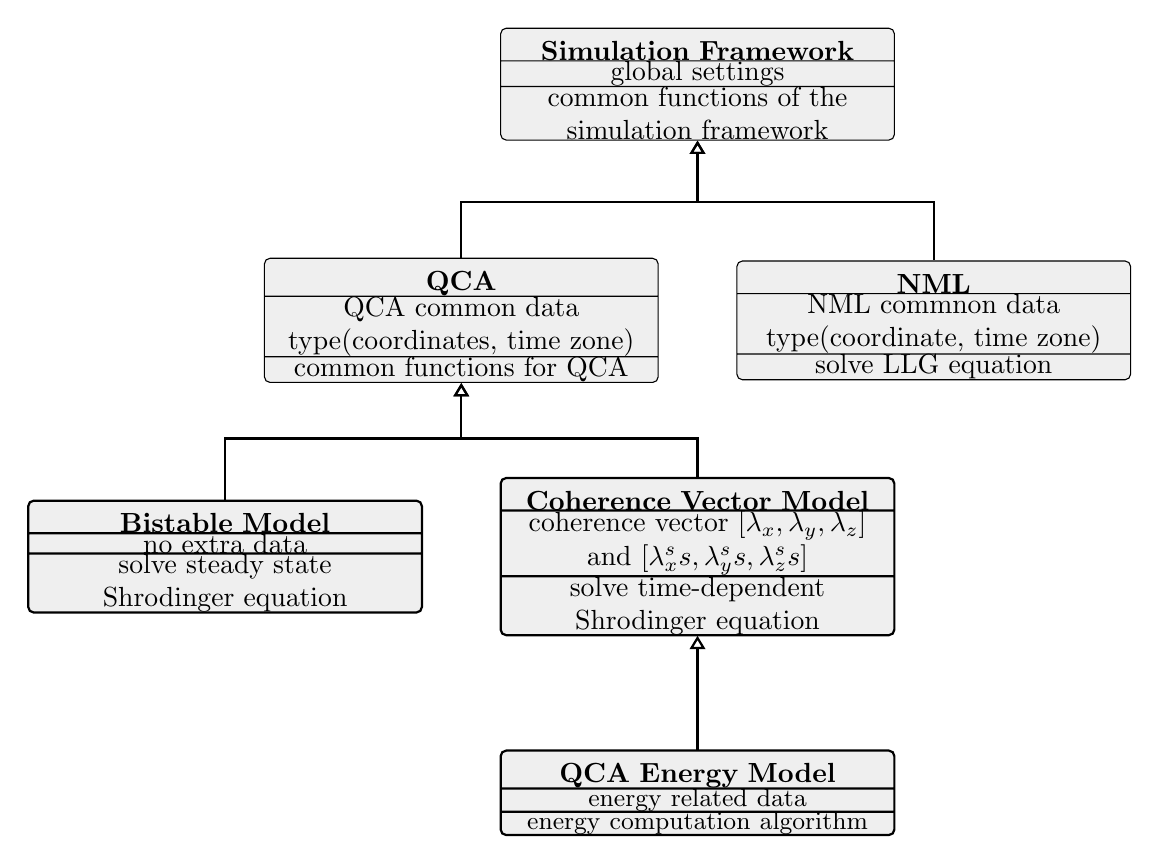
\begin{tikzpicture}[
trait/.style={ 
	rectangle split, rectangle split parts=3, rounded corners=2pt,
	inner sep=0pt, %minimum width=3.5cm, 
	draw=black,  fill=lightgray!25, 
	text width=5cm, text height=0.4cm,
	text centered,
},
edge from parent fork down,
level distance=3cm,
sibling distance=6cm,
edge from parent/.style={draw, thick,<-,>={Triangle[open]}},
] 
\node[trait] (simulation){
    \textbf{Simulation Framework}
    \nodepart{second}{global settings}
    \nodepart{third} {common functions of the simulation framework}
    }
    child {node[trait](qca){
        \textbf{QCA}
        \nodepart{second}{QCA common data type(coordinates, time zone)}
        \nodepart{third}{common functions for QCA}
        }
        child{node[trait](bistable){
            \textbf{Bistable Model}
            \nodepart{second}{no extra data}
            \nodepart{third}{solve steady state Shrodinger equation}
            }
        }
        child{node[trait] (coherence){
            \textbf{Coherence Vector Model}
            \nodepart{second} {coherence vector $[\lambda_x, \lambda_y, \lambda_z]$ and $[\lambda_x^ss, \lambda_y^ss, \lambda_z^ss]$}
            \nodepart{third}{solve time-dependent Shrodinger equation}
            }
            child{node[trait](energy){
                \textbf{QCA Energy Model}
                \nodepart{second}\small{energy related data}
                \nodepart{third}\small{energy computation algorithm}
                }
            }
        }
    }
    child{node[trait](nml){
        \textbf{NML}
        \nodepart{second}{NML commnon data type(coordinate, time zone)}
        \nodepart{third}{solve LLG equation}
        }
    }
;
\end{tikzpicture}
\end{document}
